\documentclass[12pt,letterpaper, onecolumn]{exam}
\usepackage{amsmath}
\usepackage{amssymb}
\usepackage{graphicx}
\usepackage{booktabs}
\usepackage{geometry}
\usepackage{hyperref}
\usepackage{subcaption} % For subfigures
\usepackage{minted}


% \documentclass[a4paper,12pt]{article}
% \usepackage[utf8]{inputenc}
% \usepackage[T1]{fontenc}
\usepackage{amsmath}
\usepackage{algorithm}
\usepackage{algpseudocode}
\usepackage{minted}
\usepackage{xcolor} 
% \usepackage{geometry}
% % \geometry{margin=1in}
% \usepackage{lmodern}



\lhead{College of Arts \& Sciences\\}
\rhead{Kent State University\\}
% \chead{\hline} % Un-comment to draw line below header
\thispagestyle{empty}   %For removing header/footer from page 1

\begin{document}

\begingroup  
    \centering
    \LARGE Data Mining\\
    \LARGE Assignment 3\\[0.5em]
    \large \today\\[0.5em]
    \large Viet Huy Duong\par
    \large 811433146\par
    % \large Class/Batch/Section\par
\endgroup
\rule{\textwidth}{0.4pt}     
\pointsdroppedatright   %Self-explanatory
\printanswers
\renewcommand{\solutiontitle}{\noindent\textbf{}}   %Replace "Ans:" with starting keyword in solution box

\begin{questions}

    \question[10 pts] Table 1 shows a transaction database. Please answer the following questions. \droppoints

    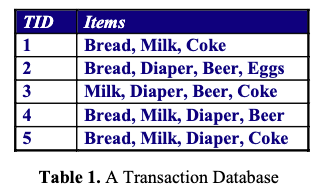
\includegraphics[width=0.5\textwidth]{figure/P1.png}

    \begin{parts}
        \part  Please enumerate all association rules involving 3 items $\{Bread, Milk, Coke\}$.
        \part Please compute the support and confidence of each association rule you listed in a.
    \end{parts}
    \newpage
    \begin{solution}


        \textbf{(a) Please enumerate all association rules involving 3 items Bread, Milk, Coke.}
        The association rules involve exactly 3 items {Bread (i will call: B), Milk (i will call: M), Coke (i will call: C)},with the antecedent and consequent parts combined being this non-empty set:
        
        \begin{itemize}
            \item \( B \rightarrow M, C \)
            \item \( M \rightarrow B, C \)
            \item \( C \rightarrow B, M \)
            \item \( B, M \rightarrow C \)
            \item \( B, C \rightarrow M \)
            \item \( M, C \rightarrow B \)
        \end{itemize}

        \textbf{(b) Please compute the support and confidence of each association rule you listed in a.}

        The total number of transaction is 5. So:

        \begin{itemize}
            \item Support of rule \( X \rightarrow Y \) = freq \( (X \cup Y) \) / total\_transaction.
            \item Confidence = support \( (X \cup Y) \) / support \( X \).
        \end{itemize}

        % Từ dữ liệu:

        According to the data:

        \begin{itemize}
            \item \( \{B, M, C\} \) is appeared at TID 1 and TID 5\(\rightarrow\) freq = 2.
            \item Partitional Freq:
            \begin{itemize}
                \item \( \{B\} = 4 \) (TID 1, 2, 4, 5)
                \item \( \{M\} = 4 \) (TID 1, 3, 4, 5)
                \item \( \{C\} = 3 \) (TID 1, 3, 5)
                \item \( \{B, M\} = 3 \) (TID 1, 4, 5)
                \item \( \{B, C\} = 2 \) (TID 1, 5)
                \item \( \{M, C\} = 3 \) (TID 1, 3, 5)
            \end{itemize}
        \end{itemize}


        \begin{itemize}
            \item \( B \rightarrow M, C \):
            \begin{itemize}
                \item Support = \( \frac{2}{5} = 0.4 \)
                \item Confidence = \( \frac{\frac{2}{5}}{\frac{4}{5}} = 0.5 \)
            \end{itemize}
            \item \( M \rightarrow B, C \):
            \begin{itemize}
                \item Support = 0.4
                \item Confidence = \( \frac{\frac{2}{5}}{\frac{4}{5}} = 0.5 \)
            \end{itemize}
            \item \( C \rightarrow B, M \):
            \begin{itemize}
                \item Support = 0.4
                \item Confidence = \( \frac{\frac{2}{5}}{\frac{3}{5}} = \frac{2}{3} \approx 0.667 \)
            \end{itemize}
            \item \( B, M \rightarrow C \):
            \begin{itemize}
                \item Support = 0.4
                \item Confidence = \( \frac{\frac{2}{5}}{\frac{3}{5}} = \frac{2}{3} \approx 0.667 \)
            \end{itemize}
            \item \( B, C \rightarrow M \):
            \begin{itemize}
                \item Support = 0.4
                \item Confidence = \( \frac{\frac{2}{5}}{\frac{2}{5}} = 1 \)
            \end{itemize}
            \item \( M, C \rightarrow B \):
            \begin{itemize}
                \item Support = 0.4
                \item Confidence = \( \frac{\frac{2}{5}}{\frac{3}{5}} = \frac{2}{3} \approx 0.667 \)
            \end{itemize}
        \end{itemize}
    \end{solution}

    \question[15 pts] 2. Please describe the anti-monotone property of the confidence for association rules, and discuss how to use this property to enable the pruning for the apriori algorithm. \droppoints
    \begin{solution}
        The anti-monotone property of confidence for association rules applies specifically to rules generated from the same frequent itemset $L$ (e.g., $L = {A, B, C}$). In this case, confidence is anti-monotone with respect to the number of items on the righthand side of the rule: as the size of the consequent ($Y$) increases (and the antecedent $X$ decreases, since $X \cup Y = L$), confidence decreases or stays the same. This is because confidence = support($L$) / support($X$), where support($L$) is fixed, and smaller $X$ leads to higher support($X$) due to the anti-monotone property of support.

        So how to use that principle to pruning in \textbf{Apriori}:

        Apriori first finds frequent itemsets based on the anti-monotone of support.

        In the rule generation phase from the frequent itemset, use the rule generation tree. Start from the rule with small consequent (1 item), calculate the confidence. If the confidence is low, prune the branch that extends the larger consequent, because the confidence will decrease. This reduces the number of rules to check, optimizes.       
    \end{solution}

    \question[40 pts] Please choose one reference paper about association rule mining from the lecture slides, and present the motivation, problem definition, and their solutions in this paper. \droppoints
    \begin{solution}
        I chose the paper: A Statistical Theory for Quantitative Association Rules by Yonatan Aumann and Yehuda Lindell, presented at the KDD-99 conference.
        

        
        \textbf{Motivation}

        % Association rules are an important data mining tool. However, many real-world databases contain quantitative attributes, and current solutions for this case are inadequate. Previous definitions, such as those of Srikant et al. (1996), used intervals to convert quantitative data into categorical data, which led to several limitations. In addition, this approach often led to exponential blowup, required a maximum support limit, and the algorithm used discretization, which lost information and only approximated the best rules. The main motivation is to introduce a new definition based on statistical inference theory, reflecting the intuition that the goal of association rules is to find extraordinary and interesting phenomena in databases, and to provide rigorous empirical evaluation on real data to demonstrate the usefulness and specificity of the mined rules.
        Problem with Traditional Association Rules: Association rules, a popular data mining tool, were originally designed for categorical data, e.g., “X → Y” with high confidence and support. Algorithms like Apriori work well for this use case. However, most real-world databases contain quantitative attributes (e.g., age, salary, height), and extending the definition of categorical to quantitative is inefficient.
      
        Limitations of previous approaches: The method of Srikant et al. 1996 \cite{srikant1996} uses intervals to discretize quantitative data, leading to:
        \begin{itemize}
            \item Inaccurate or inaccurate results (e.g., the interval [100cm, 150cm] for child height may include infants, but does not reflect the actual distribution).
            \item Exponential blowup, requiring a maxsup limit for filtering.
            \item Loss of information due to discretization, only finding an approximation of the best rule.
            \item Not capturing “interesting behavior” statistically, leading to redundant or misleading rules.
        \end{itemize}

        The authors argue that the goal of association rules is to detect extraordinary phenomena. They are inspired by categorical rules such as statistical correlations, and extend them quantitatively by using distributions instead of simple intervals. This makes it more efficient to mine real-world data, for example in the analysis of salaries, longevity, or writing habits.
        
      
      
        % Luật kết hợp là công cụ khai phá dữ liệu quan trọng, nhưng nghiên cứu chủ yếu tập trung vào cơ sở dữ liệu chỉ chứa thuộc tính phân loại (categorical data). Tuy nhiên, nhiều cơ sở dữ liệu thực tế chứa thuộc tính số lượng (quantitative attributes), và các giải pháp hiện tại cho trường hợp này chưa đầy đủ. Các định nghĩa trước đây, như của Srikant et al. (1996), sử dụng khoảng (intervals) để chuyển đổi dữ liệu số lượng thành phân loại, dẫn đến hạn chế như mô tả phân bố giá trị số lượng bị giới hạn và có thể gây hiểu lầm (ví dụ: quy tắc "height ∈ [100cm,150cm] ⇒ age ∈ [0,14]" có thể đúng nhưng không phản ánh chính xác trẻ dưới 1 tuổi ít đạt 100cm). Ngoài ra, cách tiếp cận này thường dẫn đến bùng nổ số lượng quy tắc (exponential blowup), cần giới hạn hỗ trợ tối đa (maxsup), và thuật toán sử dụng rời rạc hóa (discretization) gây mất mát thông tin, chỉ xấp xỉ các quy tắc tốt nhất. Các công trình khác như Zhang et al. (1998) cải thiện phân vùng bằng clustering, hoặc Fukuda et al. (1996) và Yoda et al. (1997) tập trung vào dự đoán hơn là luật kết hợp. Động lực chính là giới thiệu định nghĩa mới dựa trên lý thuyết suy diễn thống kê (statistical inference theory), phản ánh trực giác rằng mục tiêu của luật kết hợp là tìm hiện tượng bất thường và thú vị (extraordinary and interesting phenomena) trong cơ sở dữ liệu, đồng thời cung cấp đánh giá thực nghiệm nghiêm ngặt trên dữ liệu thực tế để chứng minh tính hữu ích và đặc trưng của các quy tắc được khai phá.
      
        \textbf{Problem Definition}

        General structure of the rule: The rule has the form “population-subset → interesting-behavior”, where:

        \begin{itemize}
            \item Left-hand side: Describes the population subset (profile), which can be a categorical attribute or a quantitative interval.
            \item Right-hand side: Describes the unusual behavior of that subset, using statistical measures of the distribution (such as mean, variance) of the quantitative attribute.
        \end{itemize}

        Interestingness: Behavior is interesting only if the distribution of the subset is significantly different from the rest of the population (complement). Use statistical tests for confirmation (e.g., Z-test for mean, F-test for variance), with confidence levels (usually 95\%) and minimum differences (mindiff) to avoid the rule of triviality.

        Specific types of rules:
        \begin{itemize}
            \item Categorical → Quantitative: Left is the categorical profile (e.g., sex = female), right is the mean/variance of one or more quantitative attributes (e.g., wage mean = \$7.90, overall = \$9.02).
            \item Quantitative → Quantitative: Left is the range on a quantitative attribute (e.g., age $\in [60,80]$), right is the mean of another quantitative attribute. Rules must be “maximal” and “irreducible” to avoid redundant rules.
        \end{itemize}

Sub-rules: Sub-rules of a basic rule, where the subset is smaller but the distribution is significantly different. This creates a hierarchy to provide comprehensive and accurate information (e.g. smoker → life expectancy = 60; smoker \& wine-drinker → life expectancy = 70).
Goal: Find all desired rules, including the basic rules and their sub-rules, without discretizing the data.

        \textbf{solution}:
        \begin{itemize}
            \item \textbf{Algorithm for Quantitative $\to$ Quantitative (one attribute to one attribute):}
            \begin{itemize}
                \item Sort the database by attribute on the left.
                \item Use \textbf{Window} procedure: Maintain two windows (regions) A (irreducible, above/below average) and B (next to expand). Traverse linearly to find maximal and irreducible regions, check Z-test to confirm.
                \item Call recursively to find sub-rules.
                \item Complexity: $O(k n \log n + k^2 n)$ with $k$ quantitative attributes, $n$ transactions. Does not depend on minimum support, runs fast even with low support.
            \end{itemize}
            \item \textbf{Algorithm for Categorical $\to$ Quantitative (many categoricals to many quantitative):}
            \begin{itemize}
                \item Step 1: Find all frequent categorical sets using Apriori.
                \item Step 2: Calculate mean/variance for each frequent set (use hash-tree, traverse only once).
                \item Step 3: Browse the lattice of frequent sets to identify basic rules and sub-rules.
            \end{itemize}
            \item Can be combined with Window for mixed profiles (categorical + a quantitative).
            \item \textbf{Statistical processing:} Use tests to filter out meaningless rules, avoid data explosion (e.g., remove 29,959 potential rules, keep only 354).
            \item \textbf{Experimental evaluation:}
            \begin{itemize}
                \item On real data: Wages (1985 CPS, 534 transactions) and Linguistics (643 transactions, on non-native English writing habits).
                \item Results: Find interesting rules (36\% according to experts), many new rules are not found by traditional statistical tools like SPSS (e.g., Russians do not use ``the'' much without source text).
                \item Compare to [7]: Their method generates more rules (about 6,000 vs 354), but only 1.2\% interesting and often misleading due to the use of intervals.
                \item Scalability: Runs fast (10--126 seconds for 10k--50k transactions), handles large data well.
            \end{itemize}
        \end{itemize}


        % The problem is to mine quantitative association rules from a database containing quantitative attributes, where the rules are of the form X $\rightarrow$ Y, where X describes a population-subset and Y describes an interesting behavior particular to that subset. The new definition is based on the distribution of the quantitative attribute, using statistical measures of mean and variance to describe the behavior.

        % A behavior is considered interesting if the distribution of the subset is significantly different from the rest of the population, confirmed by statistical tests Z-test for mean and F-test for variance, with a significance level above a user-defined threshold.

        % There are two basic types of rules:

        % \textbf{Categorical to Quantitative Rules:} On the left is the set $X \subseteq E_C \times C$ ($E_C$ is the categorical attribute, $C$ is the categorical value), defining the subset $T_X$; on the right is $\mathrm{Mean}_J(T_X)$ or $\mathrm{Variance}_J(T_X)$ ($J \subseteq E_Q$, $E_Q$ is the quantitative attribute), with $\mathrm{Mean}_J(T_X) \neq \mathrm{Mean}_J(D - T_X)$ ($D$ is the entire database), and can add $\mathrm{mindif}$ (minimum difference) to ensure minimum difference.

        % \textbf{Quantitative to Quantitative Rules:} On the left is the triplet $X = (e, r_1, r_2)$ ($e \in E_Q$, $r_1 < r_2$), defining the interval; on the right is $\mathrm{Mean}_j(T_X)$ ($j \neq e$), with the rule must be irreducible and maximal to avoid redundant rules.

        % Additionally, sub rules are defined to find basic rules and basic sub-rules recursively, avoiding contained rules that add no new information. This definition generalizes traditional classifier association rules (e.g., Agrawal et al., 1993), where confidence is equivalent to mean in the Bernoulli variable.
                    


        % Vấn đề là khai phá luật kết hợp số lượng (quantitative association rules) từ cơ sở dữ liệu chứa thuộc tính số lượng, nơi quy tắc có dạng X ⇒ Y, với X mô tả tập con dân số (population-subset) và Y mô tả hành vi thú vị (interesting behavior) đặc biệt cho tập con đó. Định nghĩa mới dựa trên phân bố giá trị (distribution) của thuộc tính số lượng, sử dụng các biện pháp thống kê như trung bình (mean) và phương sai (variance) để mô tả hành vi. Hành vi được coi là thú vị nếu phân bố của tập con khác biệt đáng kể so với phần còn lại của dân số, được xác nhận bằng kiểm định thống kê (statistical tests) như Z-test cho mean hoặc F-test cho variance, với mức ý nghĩa (significance) trên ngưỡng người dùng định nghĩa (thường 95%). Có hai loại quy tắc cơ bản:

        % Phân loại đến Số lượng (Categorical to Quantitative Rules): Bên trái là tập X ⊆ EC × C (EC là thuộc tính phân loại, C là giá trị phân loại), định nghĩa tập con TX; bên phải là MeanJ(TX) hoặc VarianceJ(TX) (J ⊆ EQ, EQ là thuộc tính số lượng), với MeanJ(TX) ≠ MeanJ(D - TX) (D là cơ sở dữ liệu toàn bộ), và có thể thêm mindif (minimum difference) để đảm bảo khác biệt tối thiểu.
        % Số lượng đến Số lượng (Quantitative to Quantitative Rules): Bên trái là triplet X = (e, r1, r2) (e ∈ EQ, r1 < r2), định nghĩa khoảng; bên phải là Meanj(TX) (j ≠ e), với quy tắc phải không thể rút gọn (irreducible) và tối đại (maximal) để tránh quy tắc thừa (redundant).

        % Ngoài ra, định nghĩa sub-rules để tìm quy tắc cơ bản (basic rules) và sub-rules cơ bản (basic sub-rules) đệ quy, tránh quy tắc chứa (contained rules) không thêm thông tin mới. Định nghĩa này tổng quát hóa luật kết hợp phân loại truyền thống (như của Agrawal et al., 1993), nơi confidence tương đương mean trong biến Bernoulli.
        % Giải pháp của họ (Their Solutions)
        % Các tác giả đề xuất khung định nghĩa và thuật toán hiệu quả để khai phá tất cả các quy tắc mong muốn (desired rules), không sử dụng rời rạc hóa mà xem thuộc tính số lượng là liên tục, tránh bùng nổ số lượng quy tắc.

        % Thuật toán cho Số lượng đến Số lượng (Quantitative to Quantitative): Sử dụng thủ tục Window để tìm quy tắc giữa hai thuộc tính số lượng i và j. Sắp xếp cơ sở dữ liệu theo i, sau đó duyệt tuyến tính để tìm vùng liên tục trên/bưới trung bình (above/below average) với hai cửa sổ A (không thể rút gọn) và B (vùng liền kề). Kết hợp A và B nếu thỏa mãn điều kiện, đảm bảo quy tắc tối đại và không thể rút gọn. Gọi đệ quy để tìm sub-rules. Độ phức tạp: O(n log n) cho sắp xếp + O(n) cho Window mỗi cặp, với n giao dịch và k thuộc tính số lượng dẫn đến tổng O(k n log n + k² n). Hỗ trợ minimum support tùy chọn để tránh quy tắc dựa trên ít dữ liệu.
        % Thuật toán cho Phân loại đến Số lượng (Categorical to Quantitative): Đúng cho bất kỳ biện pháp phân bố nào (mean, variance). Tìm tất cả quy tắc với X chứa thuộc tính phân loại và J chứa thuộc tính số lượng, không giới hạn số lượng. Sử dụng cấu trúc dữ liệu để tính toán nhanh mean/variance cho tập con, và kiểm định thống kê để xác nhận ý nghĩa.

        % Đánh giá thực nghiệm trên dữ liệu thực tế như "Determinants of Wages from the 1985 Current Population Survey" (534 giao dịch, 7 phân loại và 4 số lượng), phát hiện quy tắc như "Sex = female ⇒ Wage: mean = $7.90 p/hr (overall $9.02)" với 95% confidence. So sánh với Srikant et al. cho thấy quy tắc mới chính xác hơn, tránh hiểu lầm từ khoảng, và hữu ích cho nghiên cứu lĩnh vực (domain experts). Các vấn đề mở bao gồm mở rộng cho measures khác (median) và tối ưu hóa thuật toán.
    \end{solution}

    \question [] \droppoints
    
    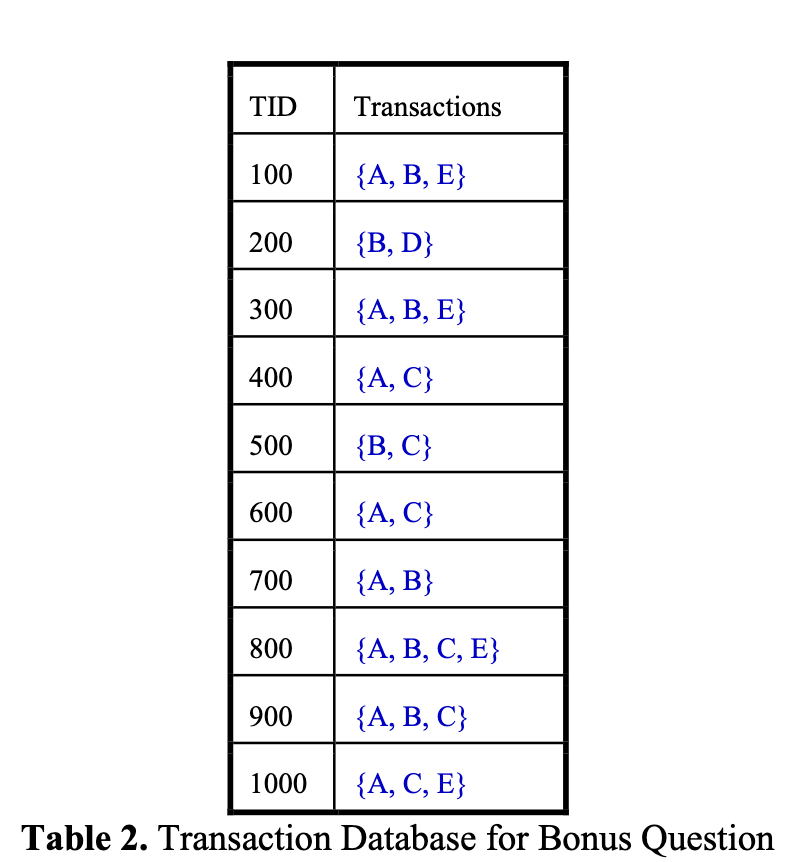
\includegraphics[width=0.6\textwidth]{figure/P4.png}
    \begin{parts}
        \part Please draw a lattice for association rules related to items {A, B, E}. [10 points]
        \part Compute the support and confidence of association rule AB → E in Table 2. [10
points]

    \end{parts}
    \begin{solution}
        \textbf{a) Please draw a lattice for association rules related to items $\{A, B, E\}$}
        
        The lattice tree:

        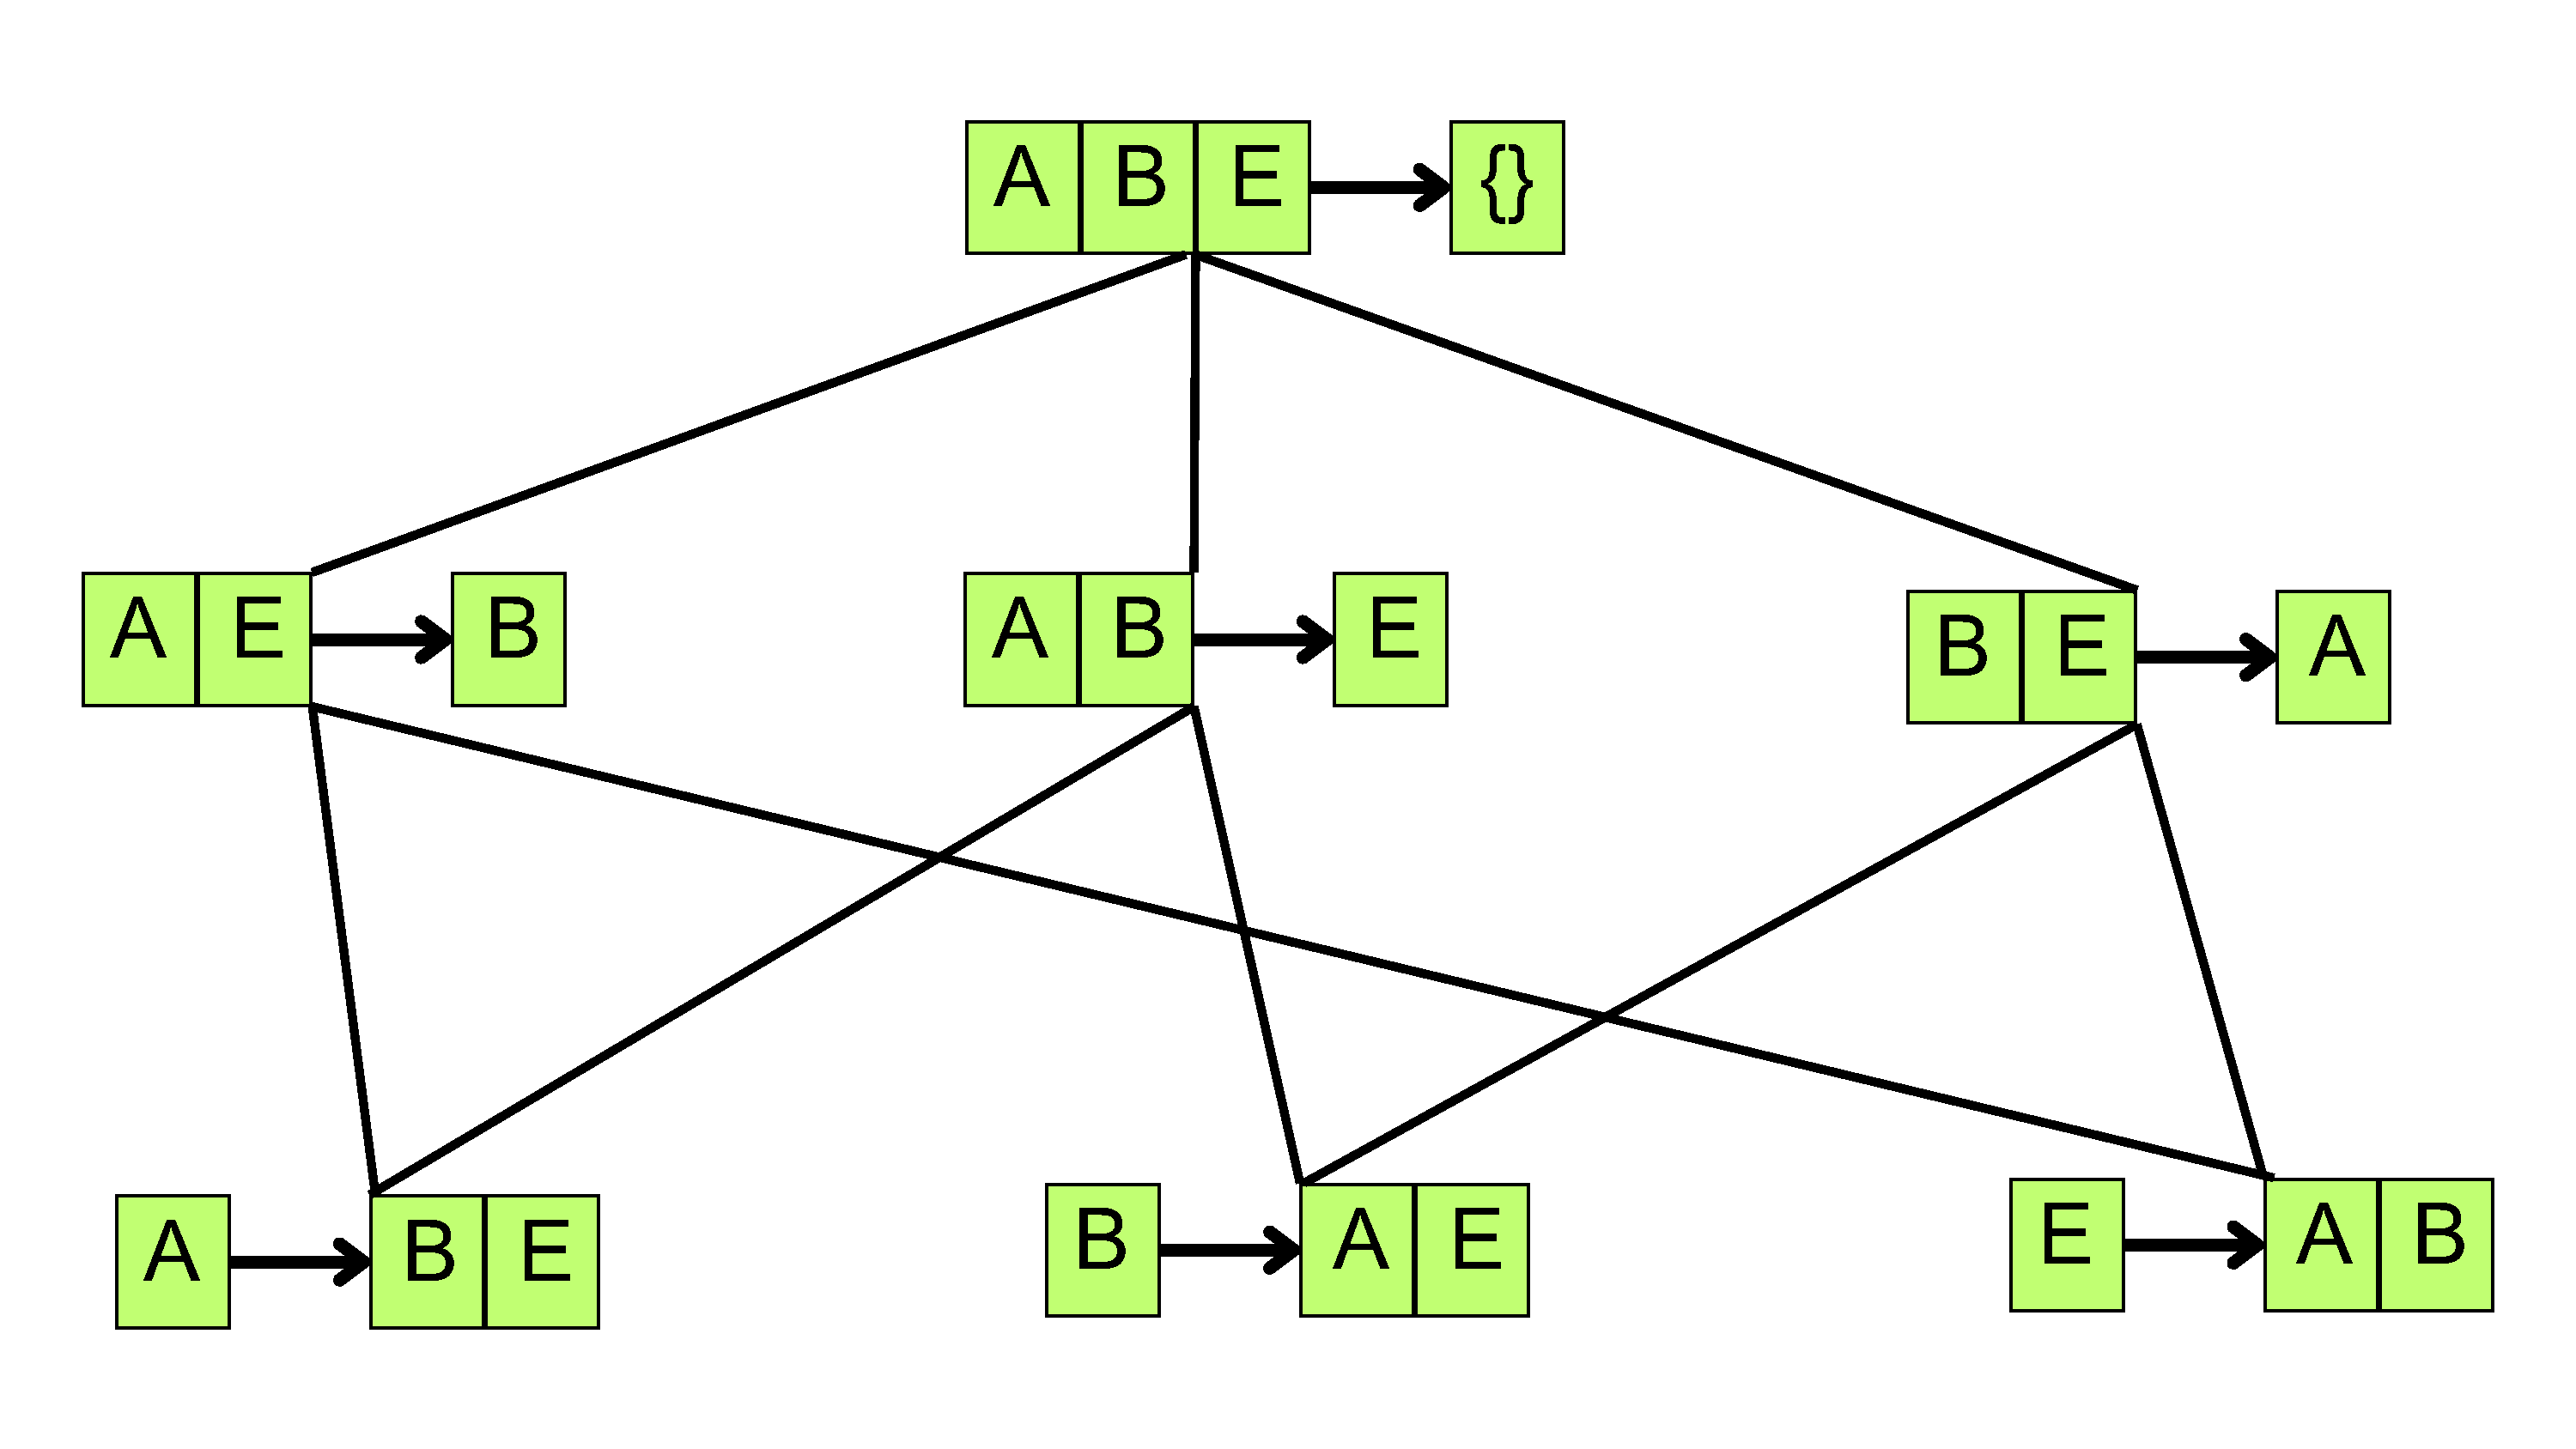
\includegraphics[width=\textwidth]{figure/Latic.pdf}
    \end{solution}

\bibliographystyle{elsarticle-num}
\bibliography{refs}

\end{questions}   
\end{document}




